\subsubsection{\stid{3.09} FFT-ECP}\label{subsubsect:fftecp}


\paragraph{Overview}

The FFT-ECP project indends to provide a sustainable 2D and 3D Fast Fourier 
Transform (FFT) library 
for distributed-heterogeneous parallel systems as the one projected for 
the upcoming exascale computing systems. FFT-ECP will leverage
established but {\it ad hoc} 
software tools that have traditionally been part of application 
codes, but not extracted as independent, supported libraries. 
These 3D FFTs rely on third-party 1D FFTs, either from FFTW or 
from vendor libraries.

The main objective of the FFT-ECP project is to:
\begin{itemize}
\item Collect existing FFT capabilities recently made available from ECP 
      application teams (LAMMPS/fftMPI and HACC/SWFFT);
\item Assess gaps and make available as a sustainable math library;
\item Explore opportunities to build 3D FFT libraries on vendor 1D and 
      2D kernels, especially leveraging on-node concurrency from 2D and 
      batched 1D formulations;
\item Focus on capabilities for Exascale platforms;
\item Emphasize leverage of vendor capabilities and addressing vendor 
      deficiencies over creation of new and independent software stack.
\end{itemize}

This effort is 
essential to providing a new and sustainable FFT software stack that 
leverages the large investment by the broader HPC community in FFT 
software. The payoff from this effort is almost guaranteed. 

FFTs are used in many applications such as molecular dynamics, 
spectrum estimation, fast convolution and correlation, signal 
modulation and many wireless multimedia applications. The 
distributed 3D FFT is one of the most important kernels involved 
in Molecular Dynamics (MD) computations and its performance can 
affect MD scalability at large scale. MD requires to solve 3D FFTs 
of medium size ($10^6--10^8$ points). The performance of the first 
principles calculations strongly depends on the performance of the 
FFT solver that performs many FFTs of size $\approx 10^7$ points in 
a calculation that we call batched FFT. Moreover, many Poisson PDE 
type of equations arising from many engineering areas such as PLASMA 
simulation, density field, etc., need to solve FFT of size above $10^9$. 

We found that more than dozen of ECP applications use FFT in their codes.
ECP applications that require FFT-based solvers suffer from the lack of 
fast and scalable 3D FFT routines for distributed-heterogeneous parallel 
systems as the ones projected for the upcoming exascale computing systems. 
To address these needs, FFT functionalities will first be delivered 
to the LAMMPS (molecular dynamics) and HACC (Hardware Accelerated
Cosmology Code) ECP applications. 
LAMMPS and HACC use their own FFTMPI and SWFFT FFT libraries, respectively.
FFT-ECP will first provide GPU-acceleration to these libraries.
The main components in the FFT-ECP framework are illustrated in 
Figure~\ref{fig:fft-ecp-pipeline}. The first and last step address the need 
for flexible FFT API to take application specific input and output (bricks/pencils), 
including arbitrary initial decompositions. The approach that we will persue for 
this step is to start from the current FFTMPI and SWFFT implementations and 
provide effient GPU support for their main communication primitives. 

\begin{figure}[htb]
    \centering
    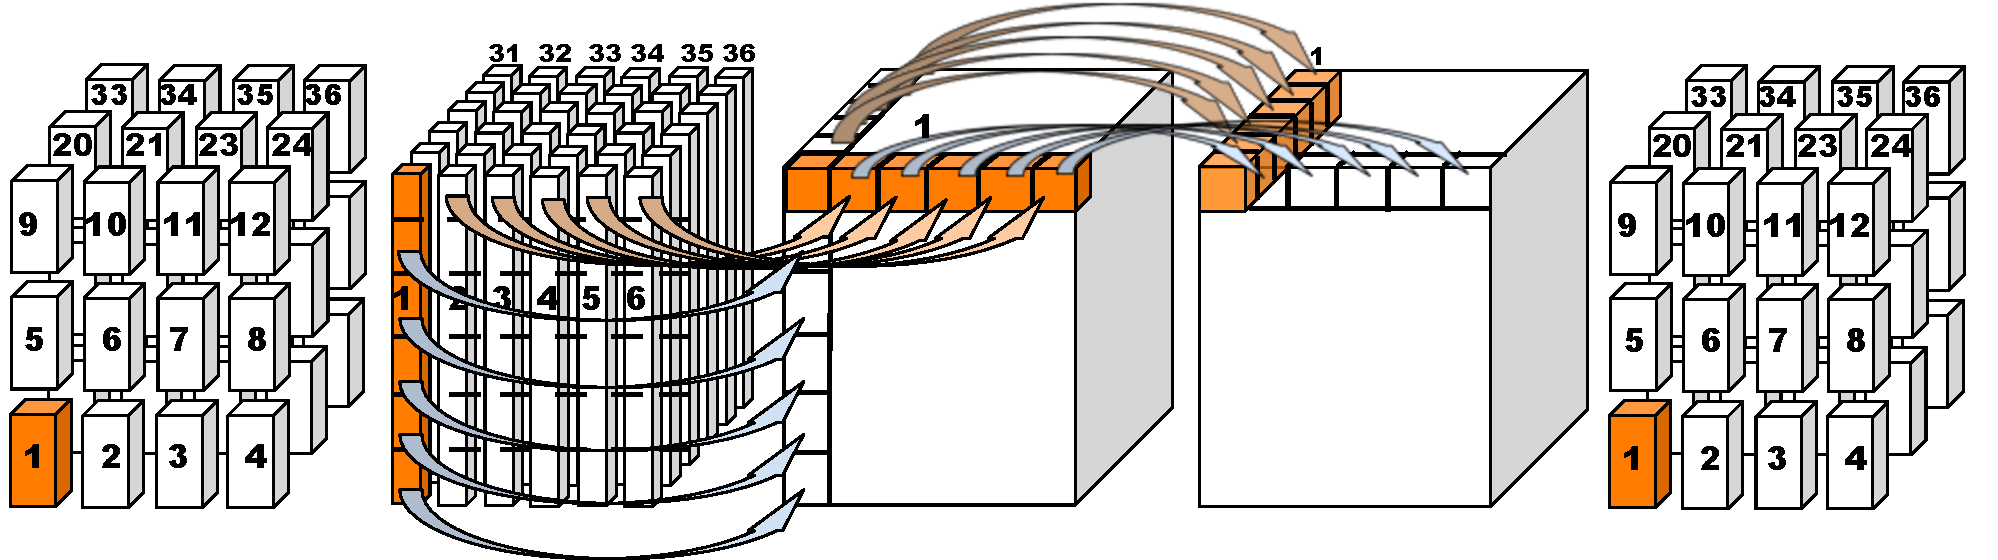
\includegraphics[width=0.75\textwidth]{projects/2.3.3-MathLibs/2.3.3.09-SLATE/ffttransormations}
    \caption{\label{fig:fft-ecp-pipeline}
    An overall 3D FFT-ECP computational pipeline:~
      1) Need flexible FFT API to take application specific input and output
         (bricks/pencils/etc., shown on the left and on right);~
      2) Need efficient packing/unpacking (on a node) and MPI communication
         routines (shown in the middle);~
      3) Need efficient 1D (or 2D in some cases) FFTs on the node (shown in the middle).}
\end{figure}

\paragraph{Key  Challenges}
\begin{enumerate}
\item
\textbf{Communication costs:}
Today's machines have very complex memory hierarchies and thus data movement, 
data layout translation, and communication should be the main focus of any 
distributed FFT library that aims to improve the performance of any ECP 
application that relies on FFT. Vendors and optimized open-source libraries 
provide very well optimized and tuned FFT routines for a single node or a 
single GPU. Therefore, although any effort on optimizing FFT kernels will 
be helpful, we prefer to target an approach that uses the available existing 
kernels and adapts them to build a more general and scalable 3D FFT library.

\item
\textbf{Appplication specifics:}
ECP applications that require FFT-based solvers suffer from the lack of fast 
and scalable 3D FFT routines for distributed-heterogeneous parallel systems 
as the ones projected for the upcoming exascale computing systems. Also, ECP 
applications may not be able to use existing FFT libraries without 
application-specific adjustments and tuning. For that, one of the main key to 
succeed with such project, is not only to study and analyze the current 
existing FFT libraries but also to study ECP application needs, study their 
FFT implementation and provide them with a suitable modular high-performance 
implementation that is flexible and easy to use and integrate in their framework.

\item
\textbf{Performance portability:}
Finally, providing many application and hardware-specific versions along with 
their parameterizations and different optimization techniques will inevitably 
create a tuning challenge. We have extensive expertize and well proven track 
record in the development and use of autotuning techniques for important GPU 
kernels. The FFT-ECP software will be linked to our autotuning tools, which 
combined with our kernels designs and use of various state-of-the-art building 
blocks will provide performance portability, software interoperability, and sustainability.
\end{enumerate}

\paragraph{Solution Strategy}

\begin{enumerate}
\item
\textbf{Evolving design:}
We will leverage vendor-optimized nodal FFT libraries as well as existing 
FFT capabilities recently made available from ECP application teams.
We will start with the fftMPI and SWFFT designs. These FFT libraries
are already integrated in ECP applications and extending them to
heterogeneous parallel systems will directly benefit the applications
and provide integrated solutions. More functionalities and application
specific optimizations will be added at a second step to support other 
ECP applications. 
\item
\textbf{Focus on communications and GPU optimizations:}
FFTs are communication bound and a main phocus in FFT-ECP is on algorithmic
design to minimize communication and efficient GPU implementations. 
Communication/computation cost and memory overhead will be analyzed and developed
for different FFT variants on current and future architecture with distributed 
and heterogeneous multi-GPU nodes. 
%Optimizing data movement as well as overlaping
%data copy with the data communication is the main bottleneck of any distributed 
%memory FFT library that must be overcommed.
\item
\textbf{Co-design with ECP application teams and vendors:}
The FFT-ECP team interacts on a regular basis with the ECP application teams
and vendors. Flexible FFT API is needed to take application specific input and 
output (bricks/pencils), including arbitrary initial decompositions. 
The APIs will be synchronized with ECP applications to be flexible, e.g., 
allowing easy construction of application-specific loading from 
and storing to arbitrary tiling of a 3D domain, data transformations from 
brick-to-pencil, pencil-to-brick, and pencil-to-pencil. Local packing and 
unpacking kernels would be accelerated leveraging GPUs' high bendwidth.
% and effient GPU transposition kernels that are already available in MAGMA.
\end{enumerate}

\paragraph{Recent Progress}
The FFT-ECP team completed an evaluation and design phase for FFTs targeting distributed 
accelerated systems. This included analysis of the current performance of FFT 
libraries and a design framework for the FFT-ECP project~\cite{thsd2018ECPFFT}. 


%The milestone delivered on the following sub-tasks:
%\begin{enumerate}
%\item Evaluation and benchmarking of current/existing FFT libraries from 
%      open-source developers and vendors;
%\item Evaluation and benchmarking of the FFT code used in other ECP 
%      applications, including LAMMPS and HACC;
%\item Study the interoperability between current vendor FFT libraries and 
%      the existing FFT library used in ECP applications, particularly for 
%      use in heterogeneous nodes with many accelerators;
%\item Propose a framework design for FFT-ECP and investigation for possible 
%      integration and/or use of vendor- developed or open-source FFT codes 
%      with our 2-D and 3-D FFT-ECP framework that emphasizes multi-GPU nodes;
%\item Analysis of the communication/computation cost and memory overhead for
%      different FFT variants and provide a study of the behavior on current 
%      and future architectures with distributed and heterogeneous multi-GPU nodes.
%\end{enumerate}

\paragraph{Next Steps}

\begin{enumerate}
\item
\textbf{Q1-Q2 FY19:}
Design and implementation phase.
\item
\textbf{Q3-Q4 FY19:}
Implementation optimization and features phase.
\end{enumerate}
